\documentclass[10pt,a4paper]{article}
\usepackage[margin=22mm]{geometry}
\usepackage[T1]{fontenc}
\usepackage{lmodern,amsmath,amssymb,graphicx,booktabs,microtype}
\usepackage[font=small,labelfont=bf]{caption}
\usepackage[hidelinks]{hyperref}
\usepackage{fancyhdr}
\pagestyle{fancy}\fancyhf{}
\fancyhead[L]{\small Computational Mechanics Projects}
\fancyhead[R]{\small StaggerLab}
\fancyfoot[C]{\thepage}
\setlength{\headheight}{14pt}
\setlength{\parindent}{0pt}\setlength{\parskip}{5pt}
\setlength{\emergencystretch}{1em}
\newcommand{\R}{\mathbb{R}}
\title{\vspace{-1.3cm}\LARGE StaggerLab: Compatible Pressure Projection and Energy Audits for Periodic Stokes Flow}
\author{\small Computational Mechanics Projects\\\small Reproducible technical research note}
\date{\small 29 September 2026}
\begin{document}\maketitle\thispagestyle{fancy}

\begin{abstract}
A pressure discretization should enforce incompressibility without introducing invisible oscillatory modes. StaggerLab combines C++17 staggered-grid difference operators with Python FFT linear solves for periodic unsteady Stokes flow. The discrete divergence and gradient are negative adjoints, yielding an orthogonal Helmholtz projection and an auditable kinetic-energy balance. Separate continuum and semidiscrete references recover spatial order 1.99979 and temporal order 2.00027. In a known decomposition, maximum divergence falls from 1.52646 to $1.59\times10^{-14}$; a forced-flow energy ledger closes within $1.20\times10^{-13}$. The study explains pressure checkerboards and distinguishes a projection potential from physical midpoint pressure.
\end{abstract}
\section{Introduction and physical model}
Staggered-grid methods place pressure and velocity at different locations to couple pressure variations directly to fluxes~\cite{mac}. Projection methods separate gradient and divergence-free velocity components~\cite{chorin}. StaggerLab studies the algebraic compatibility behind these ideas on a domain where boundaries do not obscure the mechanism. It is an original verification laboratory rather than a general Navier--Stokes solver.

For unit density and constant viscosity on $[0,L_x)\times[0,L_y)$ with periodic boundaries,
\begin{equation}
\partial_t\mathbf u=-\nabla p+\nu\Delta\mathbf u+\mathbf f,
\qquad\nabla\cdot\mathbf u=0,\qquad\langle p\rangle=0.
\end{equation}
There is no nonlinear advection. Pressure is kinematic pressure. Arrays have shape $(n_y,n_x)$ without duplicate periodic endpoints: pressure lies at $((i+1/2)\Delta x,(j+1/2)\Delta y)$; $u$ at $(i\Delta x,(j+1/2)\Delta y)$; $v$ at $((i+1/2)\Delta x,j\Delta y)$.
\section{Compatible discrete operators}
Periodic indexing defines
\begin{align}
(D\mathbf u)_{j,i}&=\frac{u_{j,i+1}-u_{j,i}}{\Delta x}
+\frac{v_{j+1,i}-v_{j,i}}{\Delta y},\\
(G_xp)_{j,i}&=\frac{p_{j,i}-p_{j,i-1}}{\Delta x},\qquad
(G_yp)_{j,i}=\frac{p_{j,i}-p_{j-1,i}}{\Delta y}.
\end{align}
Under uniform volume-weighted inner products, $G=-D^*$ and $L=DG$ is the five-point Laplacian. Its Fourier eigenvalues are
\begin{equation}
\lambda_{k,l}=-\frac{4}{\Delta x^2}\sin^2\frac{\pi k}{n_x}
-\frac{4}{\Delta y^2}\sin^2\frac{\pi l}{n_y}.
\end{equation}
Only the constant pressure is a null mode. A collocated centered gradient instead has magnitude $|\sin\vartheta|/h$, vanishing at Nyquist; the MAC face gradient has magnitude $2|\sin(\vartheta/2)|/h$, so alternating pressure is visible. This diagnoses the unstabilized stencil, not all collocated CFD methods.
\newpage
\section{Projection, time stepping, and implementation}
Solve $L\phi=D\mathbf w$ with zero mean, then set $P\mathbf w=\mathbf w-G\phi$. The FFT solver fixes the constant mode and rejects incompatible Poisson sources, allowing only a small mean consistent with its documented roundoff tolerance. Exact arithmetic gives
\begin{equation}
DP=0,\qquad P^2=P,\qquad
\tfrac12\|\mathbf w\|_h^2=\tfrac12\|P\mathbf w\|_h^2+\tfrac12\|G\phi\|_h^2.
\end{equation}
The velocity potential $\phi$ is not automatically physical pressure. For divergence-free Stokes data, applying $D$ to momentum gives $Lp=D\mathbf f$. Projecting the caller-supplied midpoint force therefore yields the physical zero-mean midpoint pressure.

Constant viscosity and periodic geometry let $P$ and $L$ commute. The projected Crank--Nicolson step is
\begin{equation}
(I-\nu\Delta t L/2)\mathbf u^{n+1}
=(I+\nu\Delta t L/2)\mathbf u^n+\Delta t P\mathbf f^{n+1/2}.
\end{equation}
Each component uses a diagonal Fourier-space Helmholtz solve. This is a finite-difference spatial discretization with an FFT solver, not spectral differentiation. The C++ kernels implement the checked stencils; pybind11 validates and copies arrays. Python handles linear solves, integration, and diagnostics. A vertex streamfunction can generate discretely divergence-free face velocities through a discrete curl, also on rectangular grids.

For midpoint velocity $\mathbf u_m$ and kinetic energy $E=\|\mathbf u\|_h^2/2$, the returned powers are $Q=-\nu\langle\mathbf u_m,L\mathbf u_m\rangle_h$ and $W=\langle\mathbf u_m,\mathbf f_m\rangle_h$. The step audit is
\begin{equation}
E^{n+1}-E^n+\Delta t(Q-W)=0.
\end{equation}
Pressure does no discrete work against solenoidal velocity. This also implies nonincreasing unforced energy, but not monotone modal amplitudes for arbitrarily large time steps.
\section{Analytical validation}
Spatial refinement uses the continuum vortex $(\sin x\cos y,-\cos x\sin y)e^{-2\nu t}$ on a square, with 12--96 cells per direction, $\nu=0.25$, and 200 steps of 0.002. Temporal refinement fixes a $24\times18$ rectangular grid and compares a discrete curl mode to $e^{\nu\lambda_{1,1}T}$ for 6--48 steps, $T=1.2$, $\nu=0.7$.
\begin{center}\begin{tabular}{lr}\toprule
Recorded diagnostic & Value\\\midrule
Finest spatial / temporal order & 1.99979 / 2.00027\\
Projection divergence before / after & 1.52646 / $1.59\times10^{-14}$\\
Known potential recovery error & $1.39\times10^{-16}$\\
Forced midpoint-pressure error & $2.22\times10^{-16}$\\
Maximum cumulative forced energy defect & $1.19\times10^{-13}$\\\bottomrule
\end{tabular}\end{center}
The forced experiment uses a $48\times32$ box, $\nu=0.12$, and 150 steps of 0.02 with vortical and gradient forcing. Further tests compare the FFT Poisson solution to an independently assembled dense matrix and check full momentum balance, adjointness, conservation, odd/even grids, and projection idempotence.
Figure~\ref{fig:results} visualizes selected recorded diagnostics.
\newpage
\begin{figure}[!ht]\centering
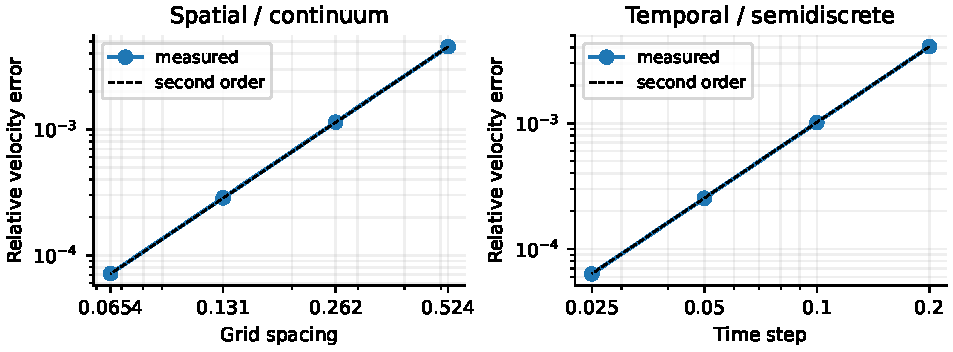
\includegraphics[width=\textwidth]{figure.pdf}
\caption{Independent spatial and temporal refinement from recorded solver outputs. Spatial errors use a continuum solution; temporal errors use a semidiscrete exponential, preventing spatial error from masking the time-integration order.}\label{fig:results}\end{figure}
\section{Discussion and limitations}
The spatial and temporal studies isolate different error sources. Near-roundoff divergence indicates satisfaction of the discrete constraint, not accuracy of an arbitrary physical flow. Likewise, recovering a deliberately prescribed discrete gradient force verifies pressure coupling without proving continuum pressure convergence for general data.

The solver is restricted to uniform periodic rectangular grids, constant viscosity, and linear Stokes physics. There are no walls, open boundaries, variable coefficients, turbulence, nonlinear advection, or adaptive steps. Crank--Nicolson is A-stable but not L-stable: large steps can weakly damp and alternate high-frequency modes. Extreme scaling is unvalidated, and all residual tolerances are floating-point diagnostics rather than interval guarantees. Array copies and FFT storage are explicit costs; no performance speedup is claimed.
\section{Reproducibility and conclusion}
This note documents the committed implementation at \texttt{497cb2b29225} and the existing synthetic results; it does not assert new solver runs. Install from the repository root with \texttt{python -m pip install ".[dev]"}; the README gives compiler requirements and verification commands. Code, data, and this manuscript are available at \href{https://github.com/racostacme-come/staggerlab}{the project repository}. No private course material is reproduced. The manuscript was prepared with AI assistance under the project owner\textquotesingle s direction; no peer review is claimed.
Run \texttt{staggerlab --output out}. Spatial and temporal CSVs, field values, the energy ledger, pressure-symbol data, and \texttt{validation.json} reproduce ten numerical acceptance checks. Compatible operators make incompressibility and energy identities mutually consistent, while independent refinement establishes the approximation order in the stated cases.
\begin{thebibliography}{9}
\bibitem{mac} F. H. Harlow and J. E. Welch, Numerical calculation of time-dependent viscous incompressible flow of fluid with free surface, \emph{Physics of Fluids} 8, 2182--2189 (1965). \href{https://doi.org/10.1063/1.1761178}{doi:10.1063/1.1761178}.
\bibitem{chorin} A. J. Chorin, Numerical solution of the Navier--Stokes equations, \emph{Mathematics of Computation} 22, 745--762 (1968). \href{https://doi.org/10.1090/S0025-5718-1968-0242392-2}{doi:10.1090/S0025-5718-1968-0242392-2}.
\end{thebibliography}

\end{document}
